\section{Week - 03}
\begin{physicsmodule}{Jan 11 - Jan 17}{RoyalBlue}
  \begin{lawbox}
    \subsection*{\sffamily\bfseries Week - 03}
    \begin{enumerate}
    \item Get ready for the Boot camp and do everything by 9:30 am. \cmark 
    \item make the rough notes and track them at VIMS-ESL and update them after coming back from the Boot camp [Fri-evening].
    \item Complete the new thicknesses inclusive plots and write the caption for them [Thu-all day].
    \item Work on writing the paper after submitting the large thickness based simulations for $\mathrm{No_{80}Fe_{20}}$ as per the paper of Panda et. al. \cite{pandaUltrafastDemagnetizationPrecession2023} [Friday all daytime].
    \item 
\end{enumerate}
  \end{lawbox}
\end{physicsmodule}
%%%%%%%%%%%%%%%%%%%%%%%%%%%%%%%%%%%%%%%%%%%%%%%%%%%%%%%%%%%%%%%%%
\subsection*{\underline{Sunday Jan 11, 2026}}
\subsection*{To do Tasks:}
\begin{enumerate}
    \item Complete the packing and go to VIMS Oral Bootcamp with Aidan. There is traveling and setting up for this Bootcamp this whole day. \cmark
\end{enumerate}
% \subsection*{Completed Tasks}
% \begin{enumerate}[\ding{52}]  % You can change the number to any dingbat symbol you want
%     \item 
% \end{enumerate}
\subsection*{Notes:}
\begin{enumerate}
    \item See the detailed things done and got from the VIMS Bootcamp in the goodnotes, Pravin/Notes-2026/Oral Bootcamp.
\end{enumerate}

% \newpage
% \section{2026 Oral Communication Bootcamp VIMS}
% The image which I have to present is,
% \begin{figure}[h!]
%     \centering
%     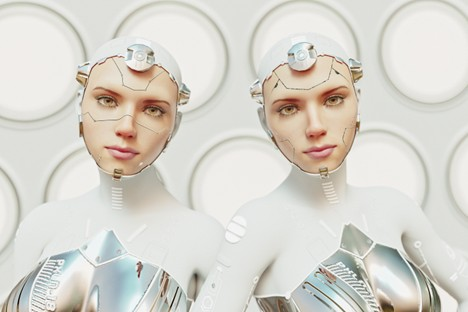
\includegraphics[width=0.95\linewidth]{Images/Pravin's pic for bootcamp.jpg}
%     \caption*{\textit{Image which Pravin Sharma is presenting in the 2026 VIMS Oral bootcamp}}
%     \label{fig:pravin-bootcamp-image}
% \end{figure}

% See the file in Goodnotes named 2026 Oral Communication Bootcamp inside January 2026. All the details are there.

%%%%%%%%%%%%%%%%%%%%%%%%%%%%%%%%%%%%%%%%%%%%%%%%%%%%%%%%%%%%%%%%%
% \subsection*{\underline{Monday Jan 12, 2026}}
% \subsection*{To do Tasks:}
% \begin{enumerate}
%     \item 
% \end{enumerate}
% \subsection*{Completed Tasks}
% \begin{enumerate}[\ding{52}]  % You can change the number to any dingbat symbol you want
%     \item 
% \end{enumerate}
% \subsection*{Notes:}
% \begin{enumerate}
%     \item 
% \end{enumerate}
% %%%%%%%%%%%%%%%%%%%%%%%%%%%%%%%%%%%%%%%%%%%%%%%%%%%%%%%%%%%%%%%%%
% \subsection*{\underline{Tuesday Jan 13, 2026}}
% \subsection*{To do Tasks:}
% \begin{enumerate}
%     \item  
% \end{enumerate}
% \subsection*{Completed Tasks}
% \begin{enumerate}[\ding{52}]  % You can change the number to any dingbat symbol you want
%     \item 
% \end{enumerate}
% \subsection*{Notes:}
% \begin{enumerate}
%     \item 
% \end{enumerate}
% %%%%%%%%%%%%%%%%%%%%%%%%%%%%%%%%%%%%%%%%%%%%%%%%%%%%%%%%%%%%%%%%%
\subsection*{\underline{Wednesday Jan 14, 2026} }
\subsection*{To do Tasks:}
\begin{enumerate}
    \item Read the papers and list the works which are supposed to be done in the remaining week.\cmark
\end{enumerate}
% \subsection*{Completed Tasks}
% \begin{enumerate}[\ding{52}]  % You can change the number to any dingbat symbol you want
%     \item 
% \end{enumerate}
% \subsection*{Notes:}
% \begin{enumerate}
%     \item 
% \end{enumerate}
%%%%%%%%%%%%%%%%%%%%%%%%%%%%%%%%%%%%%%%%%%%%%%%%%%%%%%%%%%%%%%%%%%
\subsection*{\underline{Thursday Jan 15, 2026}}
\subsection*{To do Tasks:}
\begin{enumerate}
    \item Complete the fitting for \hl{22 nm and 27 nm} for all temperatures and edit the final\_parameters table. \cmark 
    \item  PSSW waves calculations for the \hl{$\mathrm{Ni_{80}Fe_{20}}$} sample as per the paper \cite{pandaUltrafastDemagnetizationPrecession2023}.
    \begin{enumerate}[\ding{212}]
        \item The thicknesses which I am using in the benchmark simulation are only \hl{50nm and 100 nm} as per the paper.
        \item The structure is \hl{fcc, $T_c=863$K}.
        \item $\epsilon=0.790$, $z=12$, $J_{ij}=\frac{3k_BT_c}{\epsilon z}$ \\ where, $\epsilon$ is curative term derived from the mean field theory,\\ $z$ is the number of nearby atoms, \\ $T_c$ is the Curie temperature value, and \\ $k_B$ is the Boltzman constant which is $1.38\times10^{-23} J.K^{-1}$.
        \item The parameters which I have used in this simulations will be taken from the Richard Evan's paper \cite{evansAtomisticSpinModel2014}.
        \item The field application would be $15^\circ$ tilted out-of-plane (OOP).
        \item As per the external field application, which is $15^\circ$ tilted out-of-plane, the initial spin direction should also be || to the initial field. Hence, I am applying the initial spin direction as, 
        \[
        \begin{aligned}
            \mathbf{S}_0 &= (\sin\theta,\,0,\,\cos\theta) \\
            =\sin(15^\circ) &\approx 0.259 \\
            =\cos(15^\circ) &\approx 0.966 \\
            =>\mathbf{S}_0 &\approx (0.26,\,0,\,0.97)
        \end{aligned}
        \]  
        \item Submitted the simulations for \hl{$\mathrm{Ni_{80}Fe_{20}}$} for 50 nm and 100 nm.
    \end{enumerate}
\end{enumerate}
\subsection*{Completed Tasks}
\begin{enumerate}[\ding{52}]  % You can change the number to any dingbat symbol you want
    \item Completed the fitting for all the different temperatures and got some decent results also.
    \item I have put the details for the 22nm and 27 nm in the final values data set. I have to plot them, which I will do at night today. 
\end{enumerate}
% \subsection*{Notes:}
% \begin{enumerate}
%     \item 
% \end{enumerate}
% %%%%%%%%%%%%%%%%%%%%%%%%%%%%%%%%%%%%%%%%%%%%%%%%%%%%%%%%%%%%%%%%%
\subsection*{\underline{Friday Jan 16, 2026}}
\subsection*{To do Tasks:}
\begin{enumerate}
    \item Complete the replots of precessional dynamics which are required for the paper from 2 nm to 30 nm. \cmark 
    \item Complete the watching of the whole video for Heisenberg and remake the notes here in the Overleaf in the chapter \ref{chap:Magnetism/Heisenberg_Exchange}.
\end{enumerate}
\subsection*{Completed Tasks}
\begin{enumerate}[\ding{52}]  % You can change the number to any dingbat symbol you want
    \item I have completed the fitting till 30 nm and had obtained a descent trend for the increment in the $\mathrm{\alpha_{eff}}$, particularly in the case of $\mathrm{\alpha_{bulk}}$ and $\mathrm{\alpha_{surface}}$. I have a discussion for this with Rajnandini and let's see how I can write this.
    \item Got some nice looking plot for the $\mathrm{\alpha_{bulk}}$.

\end{enumerate}
% \subsection*{Notes:}
% \begin{enumerate}
%     \item 
% \end{enumerate}
% %%%%%%%%%%%%%%%%%%%%%%%%%%%%%%%%%%%%%%%%%%%%%%%%%%%%%%%%%%%%%%%%%
\subsection*{\underline{Saturday Jan 17, 2026} }
\subsection*{To do Tasks:}
\begin{enumerate}
    \item Complete the feedback form for the VIMS Oral Bootcamp attended this week earlier. \cmark
    \item Complete the Gyan Sampada video and a Lecture -02 Video for the Machine learning course.\cmark
\end{enumerate}
\subsection*{Completed Tasks}
\begin{enumerate}[\ding{52}]  % You can change the number to any dingbat symbol you want
    \item Submitted the feedback for the 2026 Oral Bootcamp at VIMS.
\end{enumerate}
% \subsection*{Notes:}
% \begin{enumerate}
%     \item 
% \end{enumerate}
\starredline



